
% \chapter{Découverte d'une source d'énergie prometteuse}
% \thispagestyle{empty}

\section{Découvertes scientifiques du début du \siecle{20}}



\begin{blockquote}
Il n'y a plus rien à découvrir en physique aujourd'hui, tout ce qui reste est d'améliorer la précision des mesures.
\end{blockquote}

\begin{wrapfigure}[15]{R}{0.5\textwidth}
\fontsize{10pt}{12pt}\selectfont
\begin{defi}[title={Thermodynamique}]
La thermodynamique est la branche de la physique qui étudie les échanges mécaniques (mouvement) et calorifiques (chaleur). Tirant son étymolgie des mots \tg{θερμός} (thermos, signifiant \emph{chaleur}) et \tg{δύναμις} (dynamis, signifiant \emph{puissance}), le mot thermodynamique a été introduit en 1864, par le physicien écossais William Thomson (Lord Kelvin).
\end{defi}
\end{wrapfigure}

Tel fut le propos que tenait Lord Kelvin en 1900. Ce dernier est révélateur de la confiance que les scientifiques de l'époque avaient dans leur compréhension du monde. Des lois paraissant inébranlables expliquaient entièrement le monde, avec les lois de Newton qui régissaient le mouvement des objets, les lois de Maxwell qui régissaient l'électricité et le magnétisme et avec trois principes qui régissaient la thermodynamique. 



Il semblait que tout était en place pour que la science puisse se concentrer sur l'amélioration des mesures et de la précision. Cependant, les années qui ont suivi ont montré que Kelvin se trompait.%

\vspace{-0.5cm}


\subsection{Découverte de la radioactivité}

\begin{wrapfigure}[12]{L}{0.3\textwidth}
    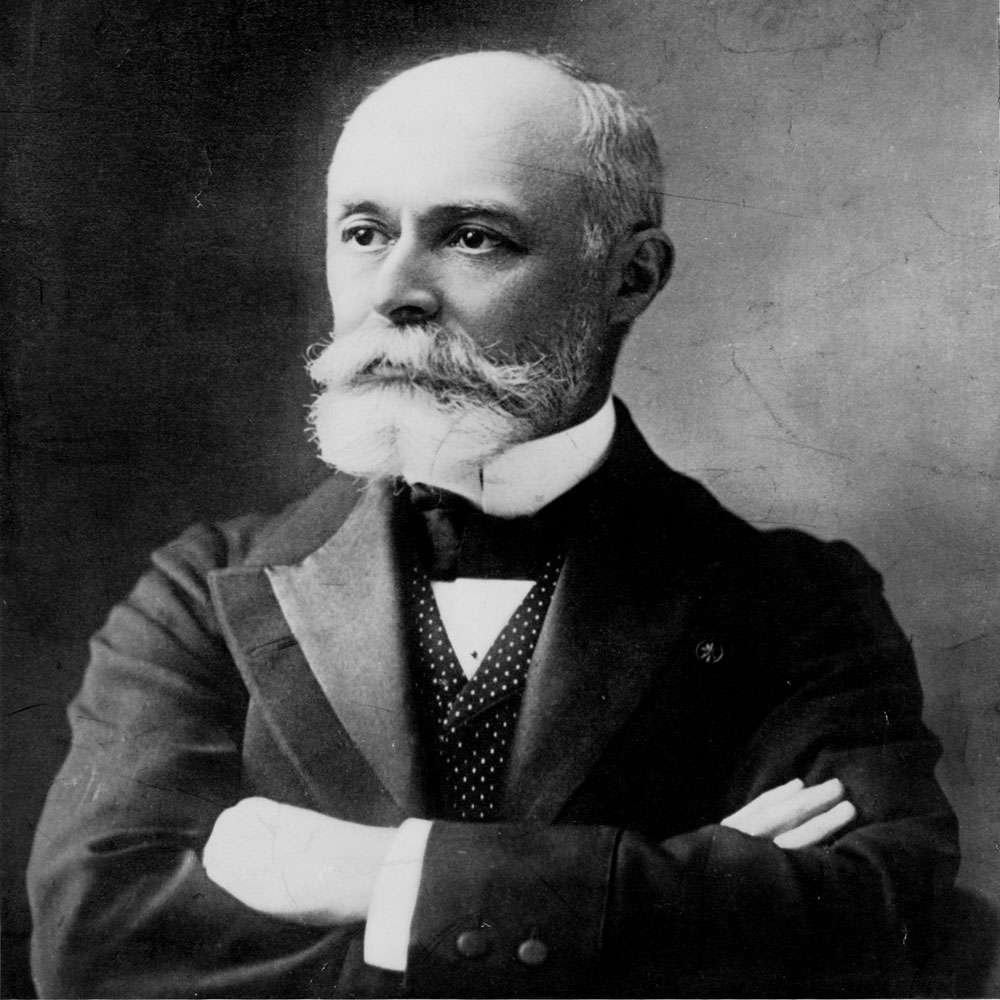
\includegraphics[width=0.3\textwidth]{images/becquerel.jpg}
    \begin{center}
        \bfseries Henri Becquerel
    \end{center}
\end{wrapfigure}


En 1896, le physicien français Henri Becquerel travaillait sur la phosphorescence, un phénomène par lequel certaines substances émettent de la lumière après avoir été exposées à la lumière. Il a exposé des sels d'uranium à la lumière du soleil, puis les a placés dans une chambre noire avec une plaque photographique. Il a découvert que la plaque photographique était brumeuse, même si les sels n'étaient pas exposés à la lumière.


\begingroup



Becquerel a d'abord pensé que la phosphorescence était responsable de l'apparition d'une image sur la plaque photographique. Cependant, il a réalisé plus tard que l'image apparaissait même si les sels n'étaient pas exposés à la lumière. Il a conclu que les sels d'uranium émettent spontanément des rayons qui peuvent traverser la matière et impressionner une plaque photographique.


Becquerel a nommé ces rayons \og rayons uraniques \fg. Il a également découvert que les rayons uraniques pouvaient ioniser l'air, ce qui signifie qu'ils pouvaient provoquer la séparation des charges électriques.


Les travaux de Becquerel ont été poursuivis par Marie et Pierre Curie, qui ont découvert deux nouveaux éléments radioactifs, le polonium et le radium. Ils ont également mis au point une méthode pour isoler le radium, qui est un élément très radioactif.

\endgroup

\begin{rmq}[title={Méthode pour isoler du radium}]
La première étape consiste à extraire chimiquement l'uranium de la pechblende, un minerai qui contient de l'uranium et du radium. 

Une fois l'uranium extrait, il est nécessaire de le séparer du radium. Pour ce faire, les Curie ont utilisé une méthode appelée « chimie radioactive » s'appuyant sur le fait que les éléments radioactifs émettent des rayons ionisants, qui peuvent être détectés par des appareils spéciaux.

Ils ont ensuite fait usage d'un appareil appelé « électroscope » pour détecter les rayons ionisants. Ils ont placé l'uranium dans un électroscope et ont observé que l'aiguille de l'électroscope se déplaçait, ce qui indiquait que l'uranium émettait des rayons ionisants.

Après ce constat, Pierre et Marie Curie ont mise en \oe{}uvre un procédé appelé « chromatographie » pour séparer le radium de l'uranium. La chromatographie est une technique qui permet de séparer des substances en fonction de leur solubilité.

Enfin, ils ont dissous l'uranium dans un solvant et ont ajouté un autre solvant qui était insoluble dans le premier solvant. Le radium est plus soluble dans le deuxième solvant que dans le premier solvant. Les Curie ont ensuite séparé les deux solvants et ont récupéré le radium dans le deuxième solvant.

Après plusieurs étapes de purification, ils ont finalement obtenu une quantité de radium pur. Cette quantité était très faible, seulement quelques milligrammes de radium pour quatre cents tonnes de pechblende.
\end{rmq}


En 1903, Marie et Pierre Curie, ainsi qu'Henri Becquerel, ont reçu le prix Nobel de physique pour leurs travaux sur la radioactivité.

\begin{minipage}{0.7\linewidth}

\textbf{\itshape Becquerel avait découvert la radioactivité en 1896, mais il ne savait pas encore ce qu'était ce phénomène. Marie Curie a repris ses travaux et a découvert que la radioactivité était due à l'émission d'énergie par certains éléments, comme l'uranium et le radium.}
    
\end{minipage}
\begin{minipage}{0.3\linewidth}
    \begin{center}
    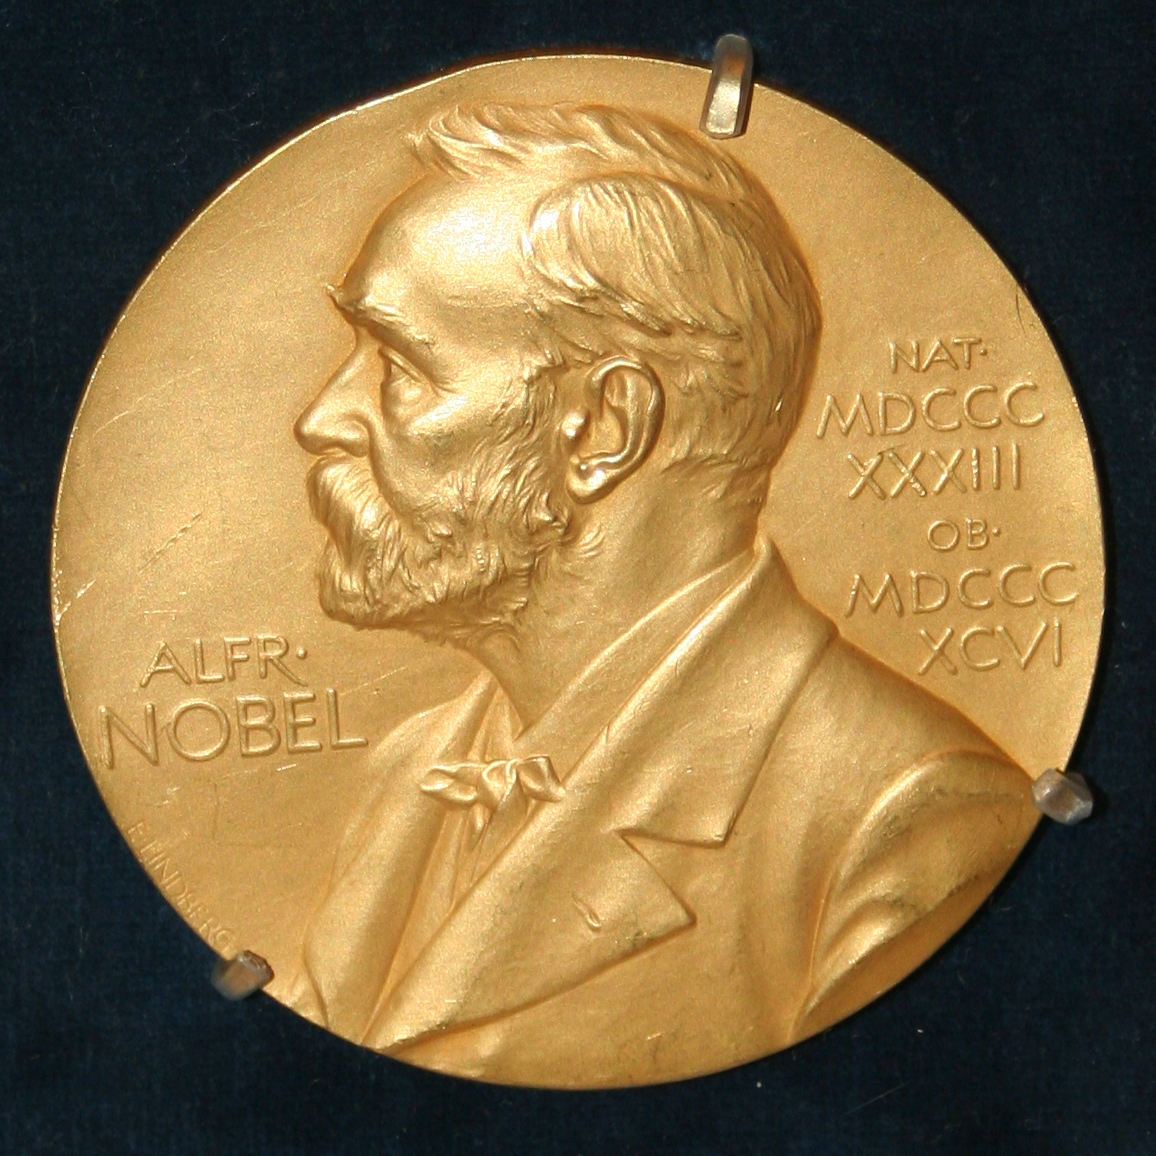
\includegraphics[width=0.8\textwidth]{images/nobel.jpg}
        \bfseries Médaille du prix Nobel
    \end{center}
\end{minipage}


\phantom i


% \begin{wrapfigure}[11]{R}{0.3\textwidth}
% \end{wrapfigure}



\begin{wrapfigure}[11]{L}{0.6\textwidth}
\begin{fact}[title={Fait historique}]
Marie Curie est devenue la première femme à recevoir un prix Nobel, et la seule à en recevoir deux, dans deux disciplines différentes. Elle a également été la première personne à recevoir deux prix Nobel en sciences.
\end{fact}
\end{wrapfigure}

\phantom i

La découverte de la radioactivité par Marie et Pierre Curie a été une étape importante dans l'histoire de la science. Elle a conduit au développement de nouvelles technologies, telles que la radiothérapie et la médecine nucléaire, dont nous parlerons plus loin.

\subsection{Grandes avancées en physique particulaire}


Les travaux des Curie ont montré que la radioactivité était due à des processus qui se déroulaient au sein des atomes. Cependant, la nature exacte du noyau atomique était encore inconnue.


\subsubsection{La découverte des particules subatomiques}

\begin{wrapfigure}[10]{L}{0.3\textwidth}
    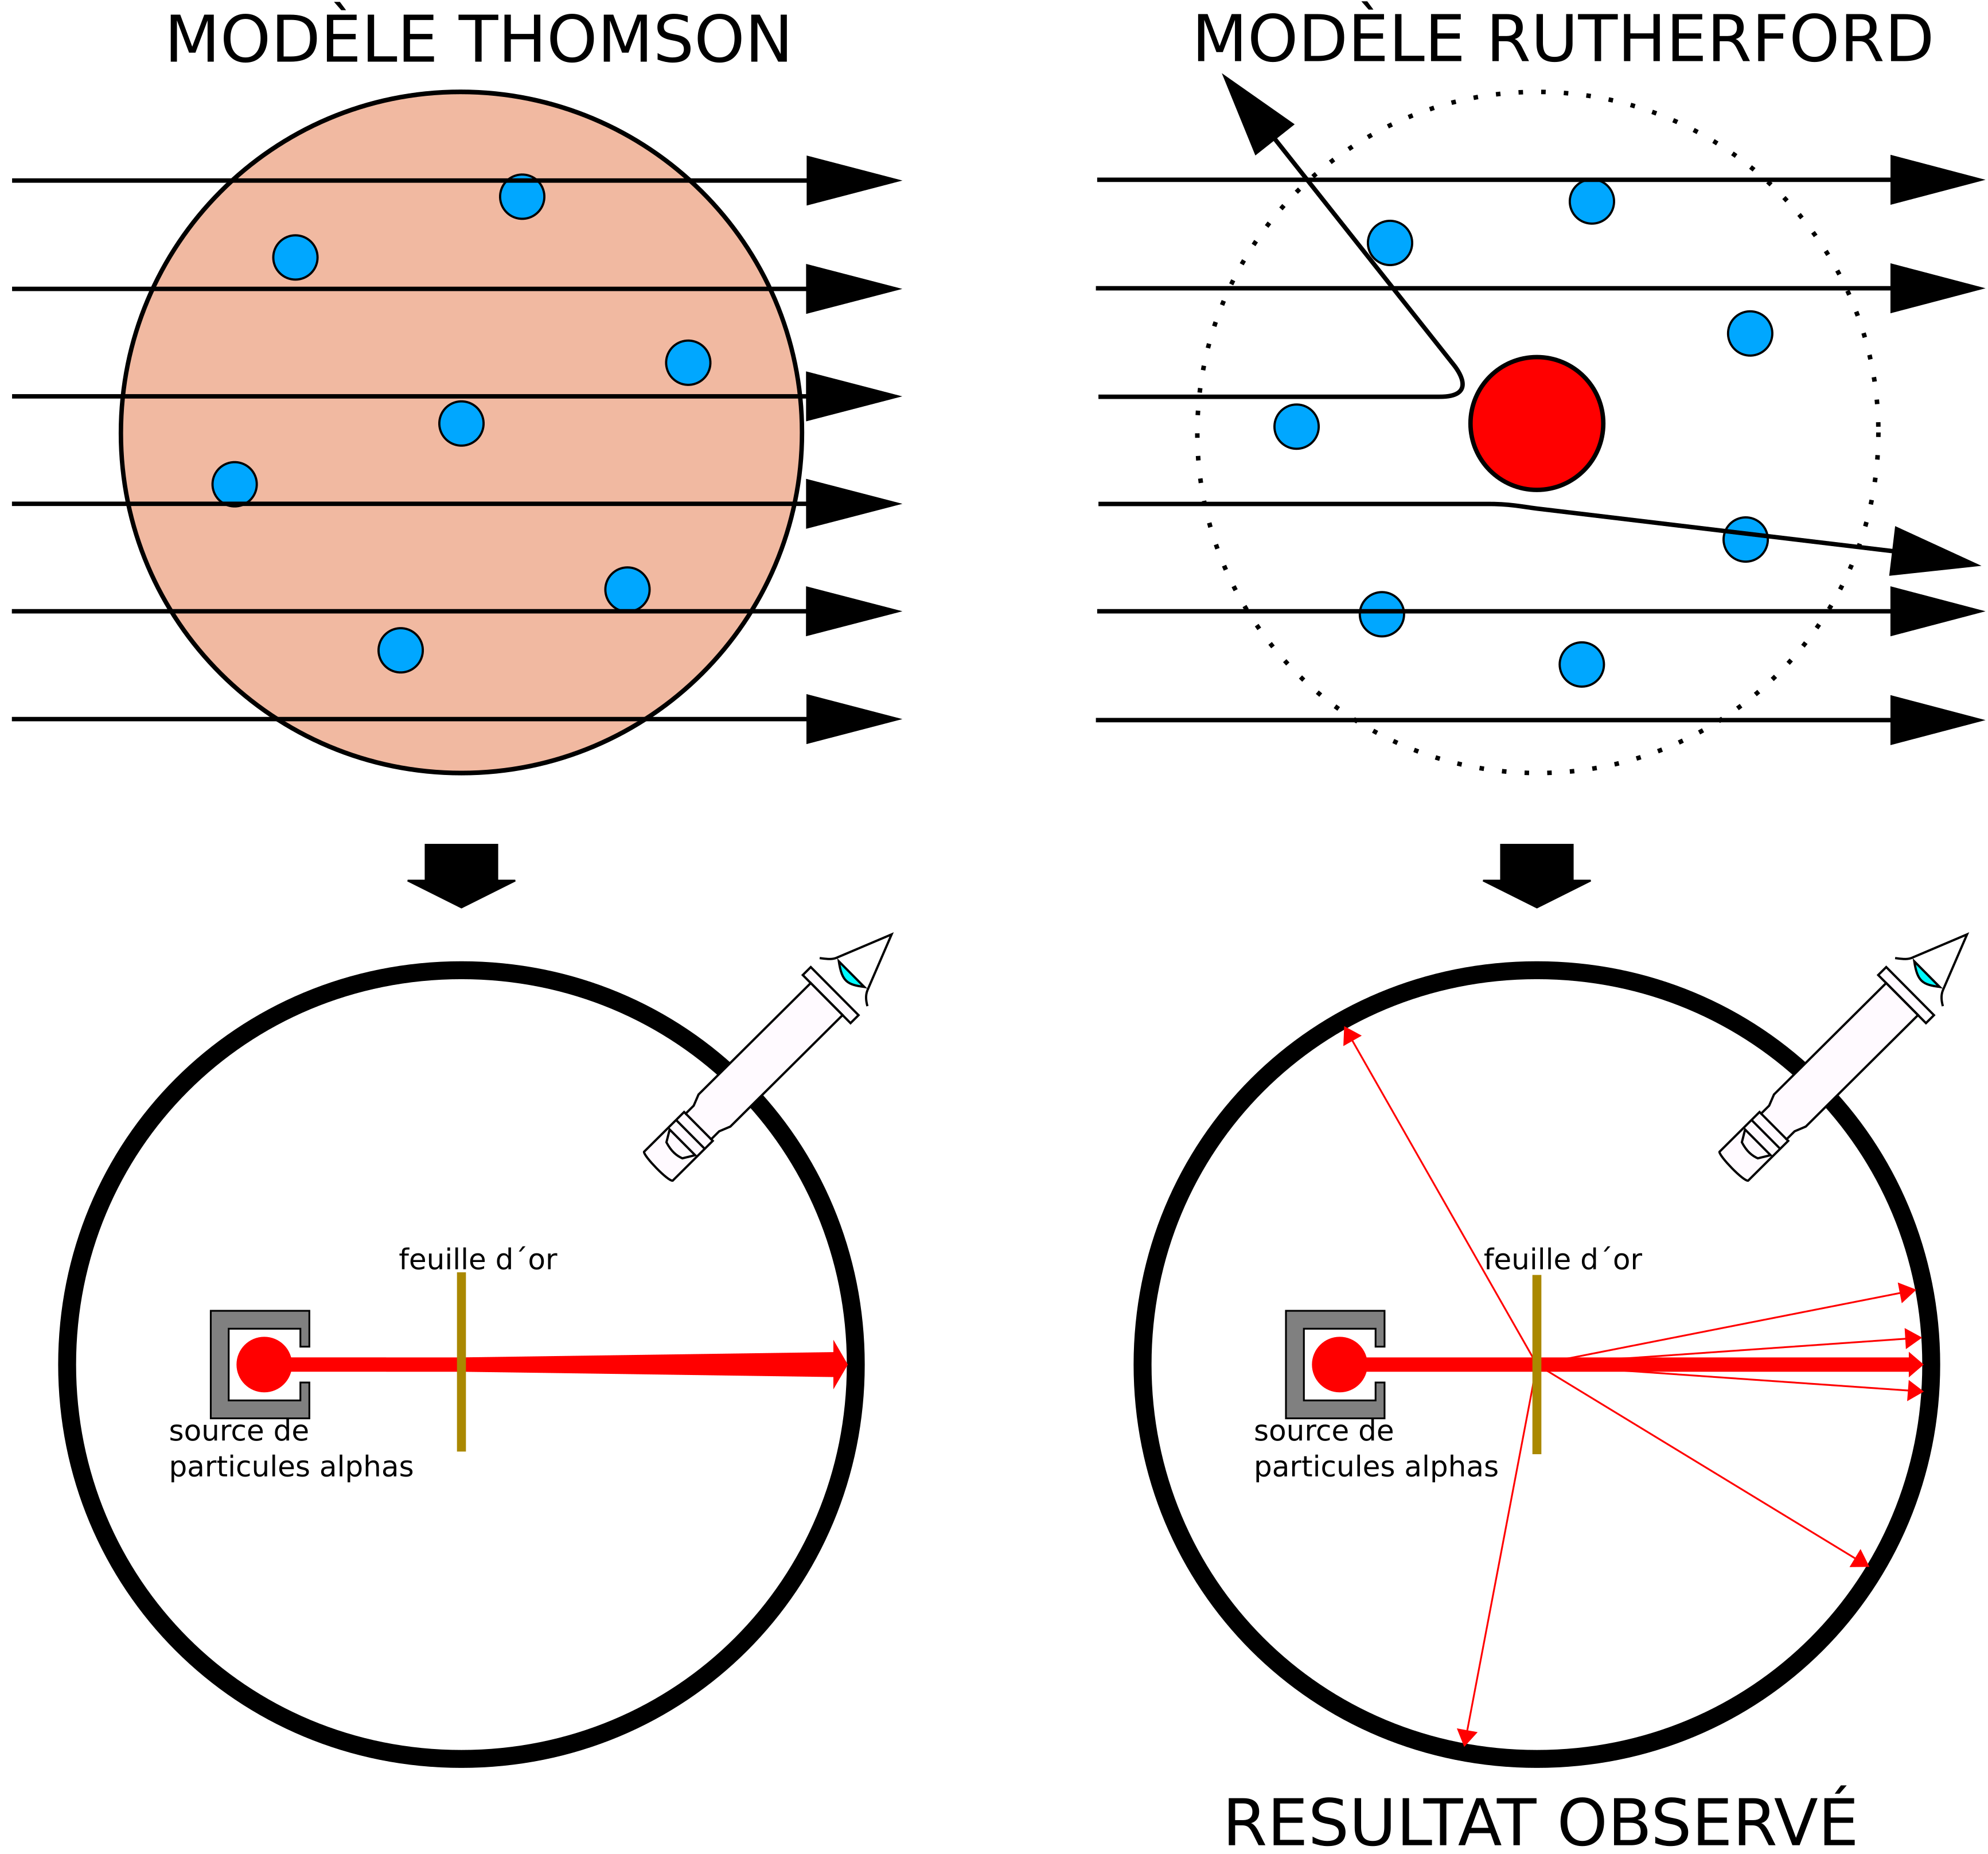
\includegraphics[width=0.3\textwidth]{images/Geiger-Marsden_experiment_expectation_and_result__French_.pdf}
    \begin{center}
        \bfseries Expérience de Rutherford
    \end{center}
\end{wrapfigure}

Ernest Rutherford, un physicien néo-zélandais du début du \textsc{xx}\up e siècle considéré comme l'un des pères de la physique nucléaire et de la chimie nucléaire, a ouvert la voie  à la découverte de nouvelles particules subatomiques. 



Rutherford est principalement connu pour son expérience de la feuille d'or, menée en 1909. Cette expérience a permis de démontrer que la matière est constituée d'un noyau dense et chargé positivement, entouré d'électrons chargés négativement. Ce modèle atomique, appelé modèle de Rutherford, a révolutionné notre compréhension de la structure de la matière.

\subsubsection{Les premiers modèles du noyau atomique}

À cette époque, la structure de l'atome était décrite par le modèle de Thomson, qui supposait que l'atome était une sphère de matière chargée positivement, avec des électrons chargés négativement répartis uniformément à l'intérieur. Cependant, cette théorie ne pouvait pas expliquer les résultats de l'expérience de Rutherford, qui montraient que certaines particules \tg{α} étaient déviées de leur trajectoire lorsqu'elles traversaient une feuille d'or.

\begin{wrapfigure}[12]{R}{0.3\textwidth}
    \includegraphics[width=0.3\textwidth]{images/Rutherford_atomic_planetary_model}
    \begin{center}
        \bfseries Structure du noyau atomique selon Rutherford
    \end{center}
\end{wrapfigure}

L'expérience de Rutherford a permis de mettre en évidence que la masse et la charge positive de l'atome sont concentrées dans un noyau central, tandis que les électrons sont répartis autour du noyau sur des orbites circulaires. Ce modèle, appelé modèle planétaire du fait de sa ressemblance avec la structure du système solaire, est encore utilisé aujourd'hui.

Le modèle atomique de Rutherford a eu un impact profond sur la science. Il a permis de comprendre la structure et les propriétés des atomes, et a ouvert la voie au développement de la chimie nucléaire et de la physique nucléaire.

Pour ses contributions à la science, Rutherford a reçu le prix Nobel de chimie en 1908.

En 1932, le physicien britannique James Chadwick a découvert le neutron, une particule sans charge électrique. En 1932 également, le physicien américain Carl Anderson a découvert le positron, une particule identique à l'électron mais chargée positivement.


Ces découvertes ont permis de comprendre que le noyau atomique était constitué de protons, de neutrons et d'électrons. Elles ont également ouvert la voie à la découverte d'autres particules subatomiques.


\subsubsection{La découverte de la fission nucléaire}

\begin{wrapfigure}[15]{L}{0.3\textwidth}
    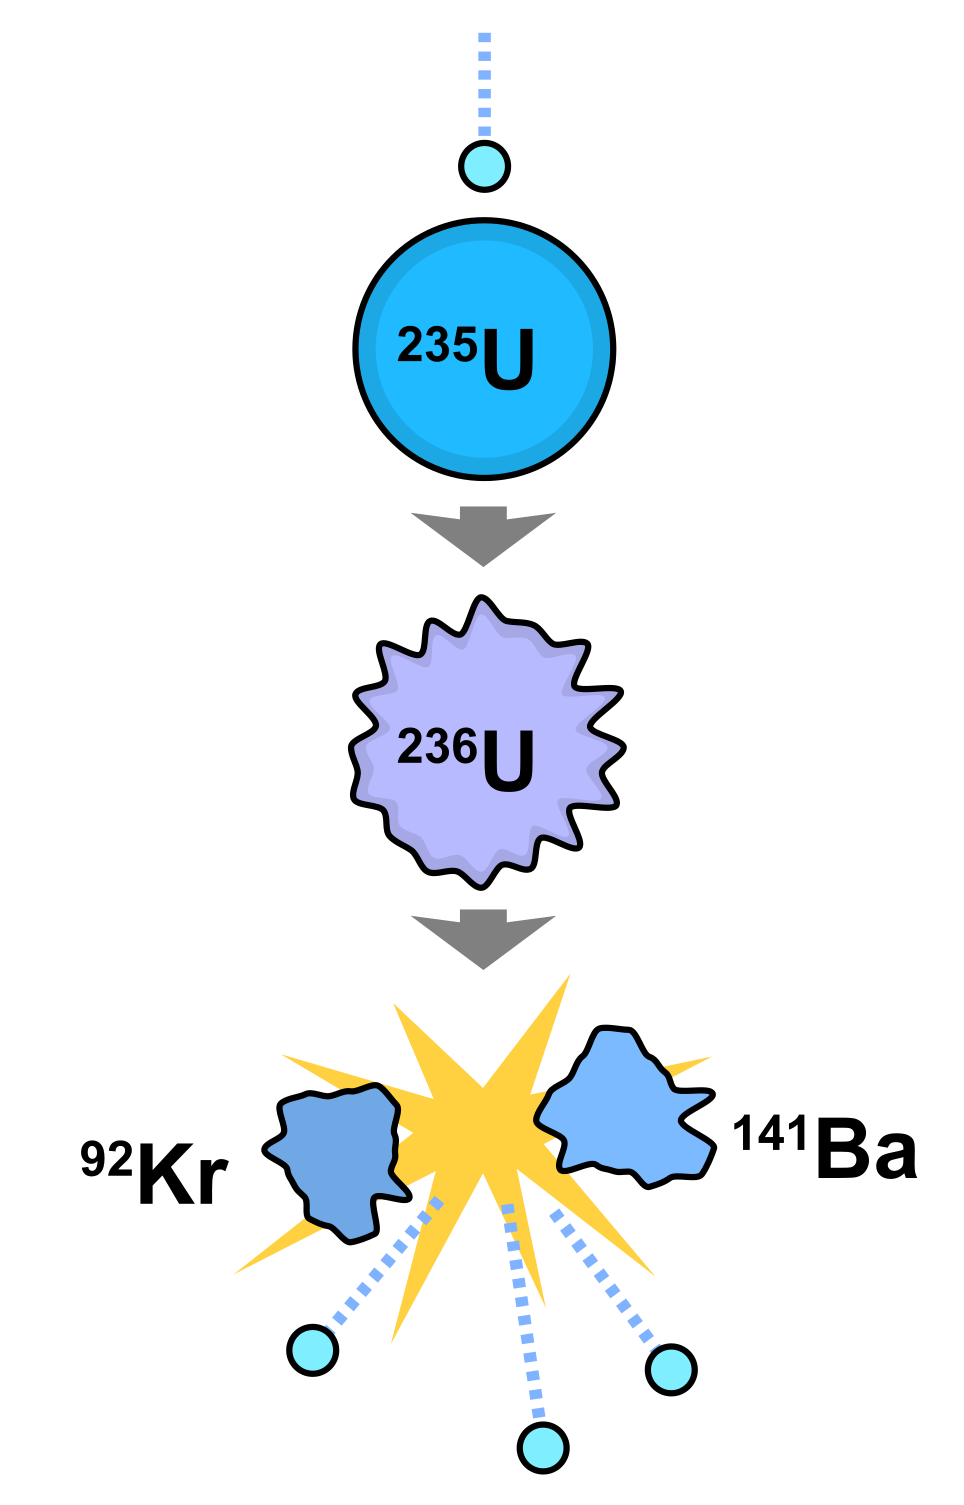
\includegraphics[width=0.3\textwidth]{images/Nuclear_fission.pdf}
    \begin{center}
        \bfseries Schéma expliquant la fission nucléaire
    \end{center}
\end{wrapfigure}

En 1938, les physiciens allemands Otto Hahn et Fritz Strassmann ont découvert la fission nucléaire, un processus dans lequel un atome lourd se divise en deux atomes plus légers. Cette découverte a conduit au développement de la bombe atomique pendant la Seconde Guerre mondiale.

\subsubsection{Le développement du modèle standard de la physique des particules}

Dans les années 1950 et 1960, les physiciens ont découvert de nombreuses nouvelles particules subatomiques. Ces découvertes ont conduit au développement du modèle standard de la physique des particules, qui est un modèle théorique qui décrit les interactions entre les particules subatomiques.

Le modèle standard est un modèle très réussi qui a permis de prédire avec précision de nombreuses propriétés des particules subatomiques. Cependant, il existe encore des questions auxquelles il ne répond pas, telles que la nature de la matière noire et de l'énergie noire.



\subsubsection{L'état de la recherche en physique des particules aujourd'hui}

Les physiciens continuent de travailler sur la compréhension de la matière et de l'énergie à l'échelle subatomique. Les recherches actuelles se concentrent sur la recherche de nouvelles particules subatomiques, la compréhension de la nature des forces fondamentales et la recherche de la théorie du tout, qui est un modèle théorique qui unifierait toutes les forces fondamentales de la nature.


\subsection{Découverte de l'énergie nucléaire}

La découverte de la fission nucléaire est une histoire qui a commencé en 1938, lorsque les physiciens allemands Otto Hahn et Fritz Strassmann ont découvert que l'uranium pouvait se diviser en deux atomes plus petits lorsqu'il était bombardé par des neutrons. Cette découverte a été une étape importante dans le développement de la technologie nucléaire et a conduit à la création de la bombe atomique.



\begin{rmq}[title=Fission nucléaire expliquée]
La découverte de la fission nucléaire est une histoire qui a commencé en 1938, lorsque les physiciens allemands Otto Hahn et Fritz Strassmann ont découvert que l'uranium pouvait se diviser en deux atomes plus petits lorsqu'il était bombardé par des neutrons. Cette découverte a été une étape importante dans le développement de la technologie nucléaire et a conduit à la création de la bombe atomique.

Hahn et Strassmann travaillaient sur la radioactivité de l'uranium lorsqu'ils ont observé que l'uranium bombardé par des neutrons produisait des éléments plus légers, tels que le baryum et le krypton. Ils ont initialement supposé que ces éléments étaient produits par la capture d'un neutron par l'uranium, mais ils ont rapidement réalisé que quelque chose de plus complexe se produisait.

Lise Meitner, une amie de Hahn qui avait fui l'Allemagne nazie, a proposé une explication de la fission nucléaire. Elle a suggéré que l'uranium pouvait se diviser en deux atomes plus petits, libérant une grande quantité d'énergie.

L'explication de Meitner a été confirmée par d'autres physiciens, dont Otto Frisch, le neveu de Meitner. Frisch a également calculé que la fission nucléaire libérait une quantité d'énergie considérable.
\end{rmq}


\section{De la radiothérapie à la médecine nucléaire}

% Dans l'ombre des débats souvent houleux entourant l'énergie nucléaire, une lueur d'utilité et d'innovation émerge, éclairant un domaine souvent méconnu du grand public : la médecine nucléaire. Au-delà des réacteurs et des centrales, le pouvoir du nucléaire trouve une application cruciale dans le domaine médical, offrant des solutions avancées et parfois révolutionnaires pour le diagnostic, le traitement et la recherche médicale. Dans cette exploration, nous plongerons dans les profondeurs de la science nucléaire, explorant comment la radioactivité, autrefois associée principalement aux risques, se transforme en un outil vital au service de la santé humaine. Loin des débats idéologiques, cette réflexion se concentrera sur les avancées médicales permises par le nucléaire, soulignant son rôle indispensable dans la compréhension des maladies, le développement de traitements innovants et la personnalisation des soins médicaux. Accompagnez-nous dans cette exploration fascinante, où les particules radioactives deviennent des alliées précieuses, redéfinissant ainsi notre compréhension de la médecine moderne.

\subsection{Ambulances de Marie Curie}

% Au cœur de la Première Guerre mondiale, une brillante scientifique allait apporter une lueur d'espoir dans l'obscurité de la tragédie. Marie Curie, double lauréate du prix Nobel, était déjà renommée pour ses découvertes révolutionnaires en radioactivité. Cependant, son engagement envers la cause médicale se révéla encore plus crucial lorsqu'elle décida de mobiliser ses connaissances pour contribuer à l'effort de guerre. C'est ainsi qu'elle introduisit la radiothérapie, une avancée médicale pionnière qui allait changer le visage du traitement des blessures de guerre.

% Pendant la Grande Guerre, les troupes étaient confrontées à des blessures d'une ampleur et d'une gravité sans précédent. Les médecins luttaient pour trouver des moyens efficaces de traiter les soldats victimes de l'horreur des combats. C'est dans ce contexte que Marie Curie, avec une détermination sans faille, mit en place des unités mobiles de radiographie sur le front. Elle utilisa des installations légères et transportables, équipées de générateurs de rayons X, pour diagnostiquer rapidement et avec précision les fractures, les éclats d'obus et les lésions internes.




% \begin{center}
%     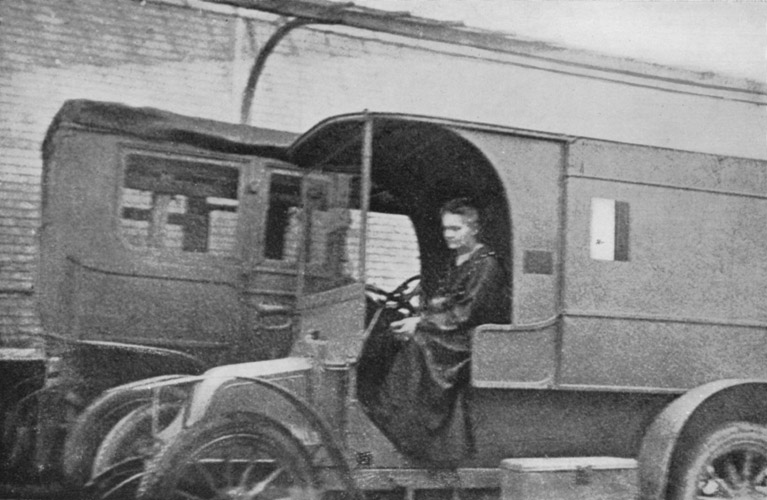
\includegraphics[width=0.8\textwidth]{images/Marie_Curie_-_Mobile_X-Ray-Unit.jpg}  
%     {\bfseries Marie Curie au volant de son ambulance}
% \end{center}

% La radiothérapie de Marie Curie ne se limita pas seulement à la détection des blessures. Elle fut également utilisée pour traiter les tissus affectés par les lésions, ouvrant ainsi la voie à une nouvelle ère dans la médecine militaire. Les rayons X, émis par les substances radioactives découvertes par Curie elle-même, démontrèrent une efficacité remarquable dans la réduction des tumeurs et dans la destruction des cellules cancéreuses.

% L'héritage de Marie Curie dans le domaine de la radiothérapie perdure aujourd'hui, rappelant comment une scientifique dévouée a pu transformer une période de conflit en une opportunité de progrès médical. Sa vision et son courage ont ouvert la voie à des traitements oncologiques modernes, établissant la radiothérapie comme l'une des armes les plus puissantes dans la lutte contre le cancer, et ce, bien au-delà des champs de bataille de la Première Guerre mondiale.



\subsection{Radiothérapie}

% \subsubsection{Présentation}

% La radiothérapie est une modalité de traitement médical qui utilise des rayonnements ionisants, tels que les rayons X, pour détruire ou endommager les cellules cancéreuses. Son objectif principal est de cibler et de détruire les cellules cancéreuses tout en minimisant les dommages aux cellules saines environnantes. La radiothérapie peut être utilisée seule ou en combinaison avec d'autres traitements, tels que la chirurgie ou la chimiothérapie, en fonction du type et du stade du cancer.

% \subsubsection{Histoire}

% La radiothérapie a ses racines dans la découverte des rayons X par Wilhelm Conrad Röntgen en 1895. Cependant, le véritable développement de la radiothérapie en tant que traitement médical a commencé au début du 20e siècle. En 1896, quelques mois après la découverte des rayons X, le physicien français Henri Becquerel a découvert la radioactivité naturelle, suivi peu de temps après par la découverte de la radioactivité artificielle par Marie et Pierre Curie.

% En 1903, le physicien allemand Hermann Müller a observé les effets néfastes des rayonnements ionisants sur les cellules biologiques. Au fil des décennies suivantes, la radiothérapie a évolué avec des avancées technologiques majeures, notamment l'invention des accélérateurs linéaires dans les années 1950, qui ont permis de délivrer des doses plus précises de rayonnements.

% \subsubsection{Importance et utilisation}

% La radiothérapie revêt une grande importance en raison de ses nombreuses applications diverses. Des exemples sont notamment

% \begin{itemize}
% \item[Traitement du Cancer] La radiothérapie est largement utilisée dans le traitement du cancer. Elle peut être utilisée pour réduire la taille des tumeurs avant la chirurgie, détruire les cellules cancéreuses résiduelles après la chirurgie, ou comme traitement principal pour les tumeurs inopérables.

% \item[Réduction des Récidives] En complément d'autres traitements, la radiothérapie contribue à réduire le risque de récidive en ciblant les cellules cancéreuses restantes après la chirurgie.

% \item[Palliation des Symptômes] Dans les cas où la guérison complète n'est pas possible, la radiothérapie peut être utilisée pour soulager les symptômes du cancer, tels que la douleur, en réduisant la taille des tumeurs.

% \item[Technologies Modernes] Les avancées technologiques ont permis le développement de techniques de radiothérapie plus précises, telles que la radiothérapie conformationnelle, la radiothérapie guidée par l'image, et la protonthérapie, réduisant ainsi les effets indésirables sur les tissus sains environnants.

% \item[Recherche et Développement] La recherche continue dans le domaine de la radiothérapie vise à améliorer l'efficacité du traitement tout en minimisant les effets secondaires. De nouvelles approches, telles que l'immunothérapie combinée à la radiothérapie, sont également explorées.
% \end{itemize}

% \subsection{Médecine nucléaire}

% \subsubsection{1930-1940 - Les premières applications médicales}

% Les années 1930 voient l'émergence des premières applications médicales de la radioactivité, notamment dans le traitement des tumeurs. En 1936, le radium est utilisé pour traiter des tumeurs de la gorge, marquant le début de la radiothérapie. Pendant la Seconde Guerre mondiale, la découverte de la scintigraphie par George de Hevesy ouvre de nouvelles perspectives pour l'imagerie médicale.

% \subsubsection{1950-1960 - L'avènement de la scintigraphie}

% Les années 1950 marquent l'avènement de la scintigraphie médicale, une technique qui utilise des traceurs radioactifs pour visualiser les organes internes. La scintigraphie permet des diagnostics plus précis et devient un outil essentiel dans la détection des maladies thyroïdiennes et la recherche de tumeurs.

% \subsubsection{1970-1980 - La tomographie par émission de positrons (TEP)}

% La découverte de la tomographie par émission de positrons (TEP) dans les années 1970 révolutionne l'imagerie médicale. La TEP permet de visualiser le métabolisme cellulaire en utilisant des traceurs radioactifs spécifiques. Elle devient cruciale dans le diagnostic précoce du cancer et dans l'évaluation de la réponse aux traitements.

% \subsubsection{1990 à aujourd'hui - Les progrès continus}

% Les avancées technologiques et la recherche constante ont permis le développement de nouvelles techniques, telles que l'imagerie par résonance magnétique (IRM) combinée à la tomographie par émission de positrons (IRM-PET), offrant des informations anatomiques et fonctionnelles simultanées. De plus, la thérapie nucléaire ciblée, utilisant des radiopharmaceutiques pour traiter spécifiquement des cellules cancéreuses, a émergé comme un domaine prometteur.

% \subsubsection{Conclusion}
% Aujourd'hui, la médecine nucléaire joue un rôle central dans le diagnostic précoce, la gestion des maladies, et la recherche médicale. Des avancées constantes dans la technologie et la compréhension des processus biologiques continuent de façonner son évolution, faisant de cette discipline une pierre angulaire de la médecine moderne.